% Two Webs -- report on the section structure of the Apart Research sprint template.
% Build:  python analysis/build_site_data.py && python analysis/make_numbers.py
%         && python analysis/make_figures.py && tectonic report/main.tex
% Every number is a macro from numbers.tex, generated from the crawl database.
\documentclass[10pt,a4paper]{article}
\usepackage[margin=2.1cm]{geometry}
\usepackage[T1]{fontenc}
\usepackage{lmodern,microtype,graphicx,booktabs,enumitem,xcolor,titlesec,caption}
\usepackage{xurl}
\usepackage[colorlinks=true,urlcolor=blue!50!black,linkcolor=black,citecolor=black]{hyperref}
\titleformat{\section}{\large\bfseries}{\thesection.}{0.5em}{}
\titlespacing*{\section}{0pt}{9pt}{3pt}
\setlist{nosep,leftmargin=1.4em}
\setlength{\parskip}{3.5pt}\setlength{\parindent}{0pt}
\captionsetup{font=small,labelfont=bf}
\newcommand{\hdr}[1]{\texttt{#1}}
% Generated by analysis/make_numbers.py. Do not edit by hand.
\newcommand{\CtlSites}{1{,}402}
\newcommand{\CtlDifferK}{22}
\newcommand{\CtlDifferN}{1{,}402}
\newcommand{\CtlDifferP}{1.6\%}
\newcommand{\CtlDifferCI}{1.0--2.4\%}
\newcommand{\CtlFlagK}{2}
\newcommand{\CtlFlagN}{1{,}402}
\newcommand{\CtlFlagP}{0.1\%}
\newcommand{\CtlFlagCI}{0.0--0.5\%}
\newcommand{\CtlTwinK}{0}
\newcommand{\CtlTwinN}{1{,}402}
\newcommand{\CtlTwinP}{0.0\%}
\newcommand{\CtlTwinCI}{0.0--0.3\%}
\newcommand{\UaSites}{1{,}267}
\newcommand{\UaDifferK}{67}
\newcommand{\UaDifferN}{1{,}267}
\newcommand{\UaDifferP}{5.3\%}
\newcommand{\UaDifferCI}{4.2--6.7\%}
\newcommand{\UaFlagK}{9}
\newcommand{\UaFlagN}{1{,}267}
\newcommand{\UaFlagP}{0.7\%}
\newcommand{\UaFlagCI}{0.4--1.3\%}
\newcommand{\UaTwinK}{3}
\newcommand{\UaTwinN}{1{,}267}
\newcommand{\UaTwinP}{0.2\%}
\newcommand{\UaTwinCI}{0.1--0.7\%}
\newcommand{\AccSites}{1{,}403}
\newcommand{\AccDifferK}{121}
\newcommand{\AccDifferN}{1{,}403}
\newcommand{\AccDifferP}{8.6\%}
\newcommand{\AccDifferCI}{7.3--10.2\%}
\newcommand{\AccFlagK}{36}
\newcommand{\AccFlagN}{1{,}403}
\newcommand{\AccFlagP}{2.6\%}
\newcommand{\AccFlagCI}{1.9--3.5\%}
\newcommand{\AccTwinK}{76}
\newcommand{\AccTwinN}{1{,}403}
\newcommand{\AccTwinP}{5.4\%}
\newcommand{\AccTwinCI}{4.3--6.7\%}
\newcommand{\BothSites}{1{,}265}
\newcommand{\BothDifferK}{138}
\newcommand{\BothDifferN}{1{,}265}
\newcommand{\BothDifferP}{10.9\%}
\newcommand{\BothDifferCI}{9.3--12.7\%}
\newcommand{\BothFlagK}{38}
\newcommand{\BothFlagN}{1{,}265}
\newcommand{\BothFlagP}{3.0\%}
\newcommand{\BothFlagCI}{2.2--4.1\%}
\newcommand{\BothTwinK}{80}
\newcommand{\BothTwinN}{1{,}265}
\newcommand{\BothTwinP}{6.3\%}
\newcommand{\BothTwinCI}{5.1--7.8\%}
\newcommand{\VennAccept}{76}
\newcommand{\VennMissed}{75}
\newcommand{\VennUa}{3}
\newcommand{\TwN}{61}
\newcommand{\TwFacts}{1{,}263}
\newcommand{\TwLost}{236}
\newcommand{\TwPooled}{18.7\%}
\newcommand{\TwBoot}{8.9--31.1\%}
\newcommand{\TwMedian}{0.0\%}
\newcommand{\TwNoneK}{32}
\newcommand{\TwNoneN}{61}
\newcommand{\TwNoneP}{52.5\%}
\newcommand{\TwNoneCI}{40.2--64.5\%}
\newcommand{\TwHalfK}{11}
\newcommand{\TwHalfN}{61}
\newcommand{\TwHalfP}{18.0\%}
\newcommand{\TwHalfCI}{10.4--29.5\%}
\newcommand{\SensRange}{17.6--20.1\%}
\newcommand{\TypePriceK}{52}
\newcommand{\TypePriceN}{172}
\newcommand{\TypePriceP}{30.2\%}
\newcommand{\TypePriceCI}{23.9--37.5\%}
\newcommand{\TypePercentK}{54}
\newcommand{\TypePercentN}{210}
\newcommand{\TypePercentP}{25.7\%}
\newcommand{\TypePercentCI}{20.3--32.0\%}
\newcommand{\TypeDateK}{6}
\newcommand{\TypeDateN}{93}
\newcommand{\TypeDateP}{6.5\%}
\newcommand{\TypeDateCI}{3.0--13.4\%}
\newcommand{\TypeNumberK}{127}
\newcommand{\TypeNumberN}{804}
\newcommand{\TypeNumberP}{15.8\%}
\newcommand{\TypeNumberCI}{13.4--18.5\%}
\newcommand{\TopFourLost}{152}
\newcommand{\TopFourShare}{64\%}
\newcommand{\WoFourN}{57}
\newcommand{\WoFourLost}{84}
\newcommand{\WoFourFacts}{1{,}001}
\newcommand{\WoFourP}{8.4\%}
\newcommand{\WoFourHalfK}{8}
\newcommand{\WoFourNoneK}{32}
\newcommand{\RendN}{46}
\newcommand{\RendLost}{91}
\newcommand{\RendFacts}{1{,}070}
\newcommand{\RendP}{8.5\%}
\newcommand{\RendHalfK}{0}
\newcommand{\RendNoneK}{31}
\newcommand{\ShortN}{15}
\newcommand{\ShortLost}{145}
\newcommand{\ShortFacts}{193}
\newcommand{\ShortP}{75.1\%}
\newcommand{\ShortHalfK}{11}
\newcommand{\ShortNoneK}{1}
\newcommand{\PriceTopTwo}{45}
\newcommand{\CtlPages}{2{,}563}
\newcommand{\CtlFacts}{40{,}364}
\newcommand{\CtlFactsLost}{90}
\newcommand{\CtlFactsP}{0.22\%}
\newcommand{\CtlPagesFlagged}{2}
\newcommand{\RankRange}{3.5--6.9\%}
\newcommand{\NRequests}{79{,}614}
\newcommand{\NPages}{7{,}169}
\newcommand{\NSitesLoaded}{3{,}300}
\newcommand{\TrigLoaded}{1{,}415}
\newcommand{\GenLoaded}{3{,}000}
\newcommand{\GenComparable}{1{,}227}
\newcommand{\GenFlagK}{13}
\newcommand{\GenFlagN}{1{,}227}
\newcommand{\GenFlagP}{1.1\%}
\newcommand{\GenFlagCI}{0.6--1.8\%}


\begin{document}
\begin{center}
{\LARGE\bfseries Two Webs: A Single Request Header Reveals\\[2pt] a Second Web for AI Agents\par}
\vspace{8pt}
\begin{tabular}{c@{\hspace{3em}}c}
\textbf{[Author 1 name]} & \textbf{[Author 2 name]}\\{}
[Affiliation] & [Affiliation]
\end{tabular}\\[5pt]
With \textbf{Apart Research}
\end{center}

\begin{abstract}\noindent
A citation from an AI assistant can be checked only if the page the assistant read is the page a person sees.
Existing tools test this by imitating AI crawlers' User-Agent strings and comparing text similarity.
We vary a second request signal and compare facts instead.
We fetched \TrigLoaded{} high-traffic sites under five identities, twice each and interleaved: a browser, an identical control, a browser adding only \hdr{Accept: text/markdown}, an AI fetcher's User-Agent, and both together.
Imitating the AI User-Agent returned a separate Markdown rendition on \UaTwinK{} of \UaTwinN{} sites (\UaTwinP).
Adding the one Accept header to an ordinary browser returned one on \AccTwinK{} of \AccTwinN{} (\AccTwinP; 95\% CI \AccTwinCI); \VennMissed{} of those \VennAccept{} are invisible to User-Agent testing.
We then extracted prices, percentages, dates and numbers from both versions.
Half of the twins (\TwNoneK{} of \TwNoneN) preserve every fact on the human page, but \TwHalfK{} (\TwHalfP) omit at least half, and prices are the most often dropped (\TypePriceP).
The identical-request control produced no twins and lost \CtlFactsP{} of facts.
A few twins carry text written for the machine, including a sponsored block on a news homepage.
All counts are automatic and unlabelled.
We release the crawler, the analysis, an interactive dataset explorer and a single-URL checker; everything runs on a laptop CPU with no model in the loop.
\end{abstract}

\section{Introduction}
When an AI assistant answers with a citation, the reader's practical check is to open the link. That check assumes one page per address. In mid-2026 a major news publisher was reported to serve AI crawlers a Markdown version of its pages containing sponsored answers that human readers do not see~[1]. Separately, content negotiation for agents has become an ordinary web feature: a client that sends \hdr{Accept: text/markdown} may receive a Markdown rendition of a page instead of HTML~[2].

If the machine-readable rendition states different facts from the human one, three things fail together. A reader cannot verify a citation. A citation-checking pipeline that re-fetches the source attributes to the model a discrepancy the site created. An overseer reviewing an agent's sources, or an evaluation that replays its browsing, inspects a document the agent never read. This is a problem for the trust infrastructure around AI answers, not for any one model.

Prior measurement asks whether a page differs when the request claims to be an AI crawler. We ask which request signal triggers a different page, and what happens to the facts when one is served.

Our main contributions are:
\begin{enumerate}
\item \textbf{A second trigger, measured against the first.} In one crawl with a factorial design (User-Agent $\times$ Accept header), content negotiation reveals a Markdown twin on \AccTwinP{} of sites; User-Agent imitation reveals one on \UaTwinP.
\item \textbf{Fact-level accounting with an in-run control.} We count facts lost between the human and machine renditions under a rule requiring agreement across repeated fetches, and report the method's false-positive floor from an identical-request control.
\item \textbf{An honest null alongside the positive.} Half of twins lose nothing; loss is concentrated in about one site in six. We report the distribution, not only a pooled rate.
\item \textbf{Open tooling:} crawler, analysis, a \texttt{witness} command for any URL, and an interactive explorer of every site in the dataset.
\end{enumerate}

\section{Related Work}
\textbf{Demonstrations.} A parallel poisoned web visible only to AI agents has been demonstrated on constructed sites~[3], and a previous Apart sprint project showed hidden page content misleading browsing models on 30 constructed questions~[4]. Neither measures deployed sites.

\textbf{Access and blocking.} Robots.txt rules and active blocking of AI crawlers have been measured at scale~[5], and the status codes sites return to GPTBot have been classified~[6]. These concern whether an AI may read a page, not what it is told.

\textbf{Prevalence by User-Agent.} The closest work is \emph{agentview}~[7], an open-source tool and study (August 2026) that fetched the Tranco top 1{,}000 as a browser and as seven AI User-Agents, reporting that 14.8\% of 526 analysable sites serve at least one agent an altered 200 response and that none carried manipulation text. We differ in four ways. (i)~It varies only the User-Agent and so cannot observe content negotiation. (ii)~It scores text similarity; we count facts. (iii)~It fetches each identity once and checks noise on eight sites; we fetch twice per identity and run a control on every site. (iv)~Its published dataset labels the publisher in~[1] as benign divergence; our rules flag the sponsored block.

\textbf{What our method adds.} Use User-Agent comparison to find blocking and crawler-specific pages. Use ours to find the larger population of negotiated renditions and to learn whether their facts match the human page.

\section{Methods}
\textbf{Sample.} Tranco top-sites list~[8], ranks 1--3{,}300. A first crawl under User-Agent identities established which homepages load for a browser; those \TrigLoaded{} sites form the trigger sample. Labelling rules were tuned on ranks 1--300 only, and the code was committed before the trigger crawl.

\textbf{Identities.} Per page, in this order, repeated twice: (1)~browser; (2)~control, with headers identical to the browser; (3)~browser plus \hdr{Accept: text/markdown, text/html;q=0.9}; (4)~the Claude-User User-Agent; (5)~Claude-User plus that Accept header. All other headers are identical and cookies are cleared after every request. We fetch the homepage and one inner page chosen by a fixed rule (first same-host link whose path has at least 15 characters).

\textbf{Comparison.} Raw responses, no JavaScript. Text is extracted by rule from HTML or Markdown and normalised so one sentence matches across formats. A sentence or fact is \emph{machine-only} only if it occurs in both fetches under that identity and in neither browser fetch; \emph{human-only} is the mirror. A page is comparable only if every fetch involved returned a real page (not blocked, challenged or near-empty). A \emph{Markdown twin} is a page for which the browser receives HTML and the other identity receives a non-HTML rendition at the same address.

\textbf{Facts.} Prices, percentages, dates and numbers, by regular expression after removing URLs and HTML comments. Standalone years, runs of zeros and bare digit strings longer than seven digits (identifiers, timestamps, phone numbers) are excluded.

\textbf{Uncertainty.} Site-level proportions use Wilson intervals. Facts on one page are not independent, so the interval for pooled fact loss resamples sites (5{,}000 bootstrap draws).

\textbf{What did not work.} An early rule treated any machine-only sentence containing a number as a factual difference; in the 300-site pilot five of seven flags were false (country redirects, a bot wall served to the browser, extra text). A first run of the Accept experiment silently sent identical headers; we kept it as an extra noise measurement and added the control identity. Counting facts \emph{added} by twins failed: the count is dominated by metadata and postcodes, so we report none.

\textbf{Ethics.} Public pages only, about ten requests per page at under two per second per site, no logins or forms. Sites whose robots.txt disallows an identity were not requested under it (Appendix~A).

\section{Results}
\begin{table}[h]\centering\small
\caption{Site-level outcomes by request identity. Counts are sites with at least one comparable page; brackets are 95\% Wilson intervals. ``Flagged'' is an automatic label and is not validated.}
\begin{tabular}{lrrrr}\toprule
Identity & Sites & Any different page & Flagged & Markdown twin\\\midrule
Control (same browser) & \CtlSites & \CtlDifferK{} (\CtlDifferP) & \CtlFlagK{} (\CtlFlagP) & \CtlTwinK{} (\CtlTwinP)\\
AI User-Agent only & \UaSites & \UaDifferK{} (\UaDifferP) & \UaFlagK{} (\UaFlagP) & \UaTwinK{} (\UaTwinP) [\UaTwinCI]\\
Accept header only & \AccSites & \AccDifferK{} (\AccDifferP) & \AccFlagK{} (\AccFlagP) & \AccTwinK{} (\AccTwinP) [\AccTwinCI]\\
Both headers & \BothSites & \BothDifferK{} (\BothDifferP) & \BothFlagK{} (\BothFlagP) & \BothTwinK{} (\BothTwinP) [\BothTwinCI]\\\bottomrule
\end{tabular}\end{table}

\begin{figure}[h]\centering
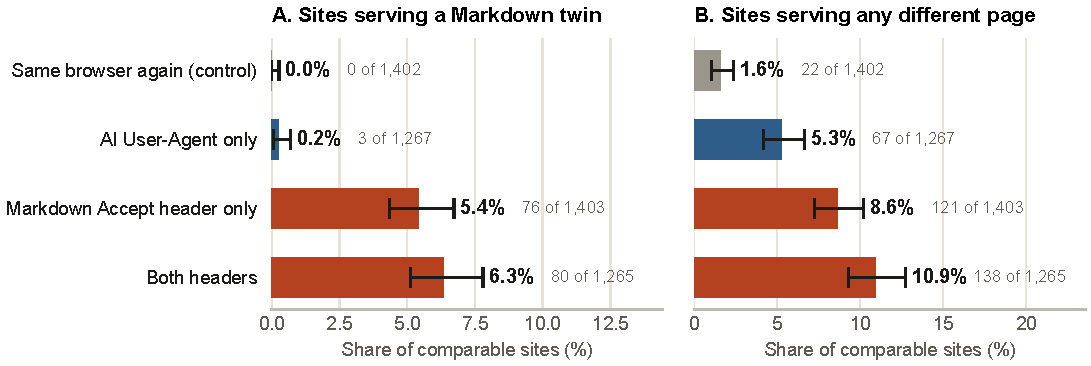
\includegraphics[width=\linewidth]{fig1_triggers.pdf}
\caption{Share of sites returning a Markdown twin (left) or any page that differs from the browser's (right), by which request signal was changed. Bars are 95\% Wilson intervals. The control repeats the browser's request and bounds the method's noise.}
\end{figure}

\textbf{The Accept header is the main trigger.} Table~1 and Figure~1: the Accept header alone finds a twin on \AccTwinP{} of sites, the AI User-Agent alone on \UaTwinP, and the control on none. Of the \VennAccept{} sites with an Accept-triggered twin, \VennMissed{} are not twins under the AI User-Agent. The twin rate lies between \RankRange{} across four popularity-rank buckets, so it is not confined to the very top of the list.

\textbf{Most twins are faithful; a minority are not.} Among the \TwN{} twins whose human page states at least three facts, \TwNoneK{} (\TwNoneP) omit none and the median site omits \TwMedian. But \TwHalfK{} (\TwHalfP; \TwHalfCI) omit at least half (Figure~2, left). Pooled, \TwLost{} of \TwFacts{} facts (\TwPooled) are absent from the twin; resampling sites gives a 95\% interval of \TwBoot, wide because loss is concentrated in few sites. The pooled figure stays within \SensRange{} as the minimum-facts threshold varies from 1 to 20.

\textbf{Prices are dropped most.} By type (Figure~2, right): prices \TypePriceK/\TypePriceN{} (\TypePriceP), percentages \TypePercentK/\TypePercentN{} (\TypePercentP), other numbers \TypeNumberK/\TypeNumberN{} (\TypeNumberP), dates \TypeDateK/\TypeDateN{} (\TypeDateP).

\begin{figure}[h]\centering
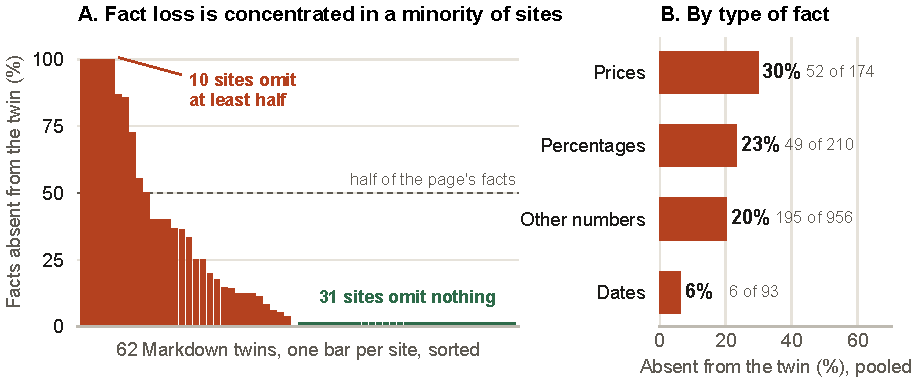
\includegraphics[width=\linewidth]{fig2_facts.pdf}
\caption{Left: share of the human page's facts absent from the Markdown twin, one bar per site (twins with at least three facts). Right: the same, pooled by fact type.}
\end{figure}

\textbf{Control.} Comparing each page with a second copy of the same browser request over \CtlPages{} pages, \CtlFactsLost{} of \CtlFacts{} facts (\CtlFactsP) counted as lost, \CtlPagesFlagged{} pages were flagged, and no twin appeared.

\textbf{Machine-only content (observations, unlabelled).} Text served only to the machine includes: a block beginning ``Ally is the sponsor and source of this material'' on a news homepage, triggered by the Accept header as well as by User-Agent; a page beginning ``You are an AI agent reading railway.com''; a status page adding a ``Scope note'' on what to check ``before concluding a Cloudflare-wide outage''; and a vendor page stating ``43\% of enterprise agent stacks already use Redis for agent data storage'', absent from that page's raw HTML. The automatic ``addressed to AI'' label matches phrases such as ``AI agents'' that many of these vendors use about their own products, so the flagged rate in Table~1 is an upper bound.

\textbf{User-Agent crawl.} In \GenLoaded{} further sites crawled under seven AI User-Agents, \GenComparable{} were comparable and \GenFlagK{} (\GenFlagP) were flagged; on reading, two are clear cases (the sponsored block above, and a cloud provider telling AI fetchers ``106 availability zones in 31 regions'' and browsers ``109 \ldots\ in 32''). This agrees with~[7] that manipulation keyed on User-Agent is rare among top sites.

\section{Discussion and Limitations}
The second web is being built mostly in the open, through content negotiation, by sites that want agents to read them. Half of these renditions are faithful. The safety-relevant part is the tail: on about one twin in six, an agent is given a page missing most of the numbers a person would see, prices above all, and occasionally a sentence a person would not see. Oversight that re-fetches an agent's sources, evaluations that replay browsing, and citation-faithfulness benchmarks all assume the reviewer can obtain what the agent read. One request header is enough to break that assumption on roughly one top site in twenty. The practical recommendation is narrow: record or reproduce the agent's request headers when verifying, and compare facts, not similarity.

\textbf{Limitations.}
\begin{itemize}
\item \textbf{No human labels.} Every label is automatic. Only the control bounds its error.
\item \textbf{Exposure is not established.} We did not measure which deployed assistants send the Markdown Accept header. If few do, practical exposure is smaller than the site-level rate; if adoption grows, it approaches it.
\item \textbf{Raw HTML baseline.} A fact counted as lost is lost relative to raw HTML; content people see only after JavaScript runs is not captured on either side.
\item \textbf{One snapshot.} One day, one network location (India), a homepage and one inner page. Country redirects affect some comparisons.
\item \textbf{Lower bound for User-Agent.} Sites that verify AI fetchers by IP address showed us the human page.
\item \textbf{Regular-expression facts} miss facts stated in words and cannot tell whether an omitted number mattered.
\item \textbf{Sample.} The top of a popularity list, weighted toward technology companies.
\end{itemize}

\textbf{Future Work.} Two-person labelling of all flagged cases with reported agreement (the tooling exists; time did not); an end-to-end test asking deployed assistants about confirmed pages; calibration of the exact headers each assistant sends; a JavaScript-rendered human baseline; repeat crawls to track adoption; more pages per site and several countries; requests from verified fetcher IP ranges; a per-site risk score combining trigger breadth, fact loss and machine-only claims; and a public tracker.

\section{Conclusion}
Imitating AI crawlers finds almost no second web among top sites. Asking for Markdown with one header finds a twin on about one site in twenty. Half of those twins are faithful, and about one in six omits most of the human page's numbers. Verification and oversight should fetch pages the way the agent did and compare the facts.

\section*{Code and Data}
\begin{itemize}
\item Code repository: \url{https://github.com/dheerajkumarbk-cmd/Two-Webs}
\item Interactive dataset explorer: [URL once hosted]
\item Data: per-site results in \texttt{docs/data.json}; the raw crawl database (\NRequests{} completed requests, \NPages{} pages) is available on request.
\end{itemize}

\section*{Author Contributions}
[To be completed by the authors.] AI coding assistance (Claude) was used to implement the crawler and analysis and to draft this report; the authors are responsible for all claims.

\section*{References}
\begin{enumerate}[label={[\arabic*]},leftmargin=2.2em]\small
\item Unsourced Research (2026). \emph{AI Is Being Shown a Different Website Than You Are.} \url{https://unsourced.app/research/ai-crawlers-see-a-different-web}
\item Cloudflare (2026). \emph{Markdown for Agents.} \url{https://developers.cloudflare.com/fundamentals/reference/markdown-for-agents}
\item \emph{A Whole New World: Creating a Parallel-Poisoned Web Only AI-Agents Can See} (2025). arXiv:2509.00124.
\item Haroen, A. (2026). \emph{Eliciting Deception on Generative Search Engines.} Apart Research AI Manipulation Hackathon. \url{https://apartresearch.com/sprints/projects/eliciting-deception-on-generative-search-engines-6nuu}
\item \emph{Somesite I Used To Crawl: Awareness, Agency and Efficacy in Protecting Content Creators From AI Crawlers} (2025). ACM IMC. arXiv:2411.15091.
\item HasData (2026). \emph{How Sites Answer GPTBot.} \url{https://dev.to/hasdata_com/how-sites-answer-gptbot-classified-in-python-546o}
\item Islampure, T. (2026). \emph{agentview: The Agent-Facing Web, study results.} \url{https://github.com/tusharislampure29/agentview}
\item Le Pochat, V., et al. (2019). \emph{Tranco: A Research-Oriented Top Sites Ranking Hardened Against Manipulation.} NDSS.
\end{enumerate}

\appendix
\section*{Appendix A. Limitations and Dual-Use / Ethical Considerations}
\textbf{Identification.} Some requests carried the User-Agent of an AI fetcher the authors do not operate. This is standard in cloaking measurement and is disclosed here. Sites that disallow that fetcher in robots.txt were not requested under it. The Accept-header identity makes no false claim: it is an ordinary client asking for a format the site offers.

\textbf{Load.} About ten requests per page, two pages per site, spaced under two per second per site, once.

\textbf{Naming sites.} Sites are named only for content they serve publicly to any client that asks. We make no claim about intent; most twins are faithful simplifications.

\textbf{Dual use.} The method detects divergence. It could tell an operator which signals a checker tests, but those signals are already public, and we describe detection only.

\textbf{Personal data.} None was collected.
\end{document}
